\chapter{Goal}
    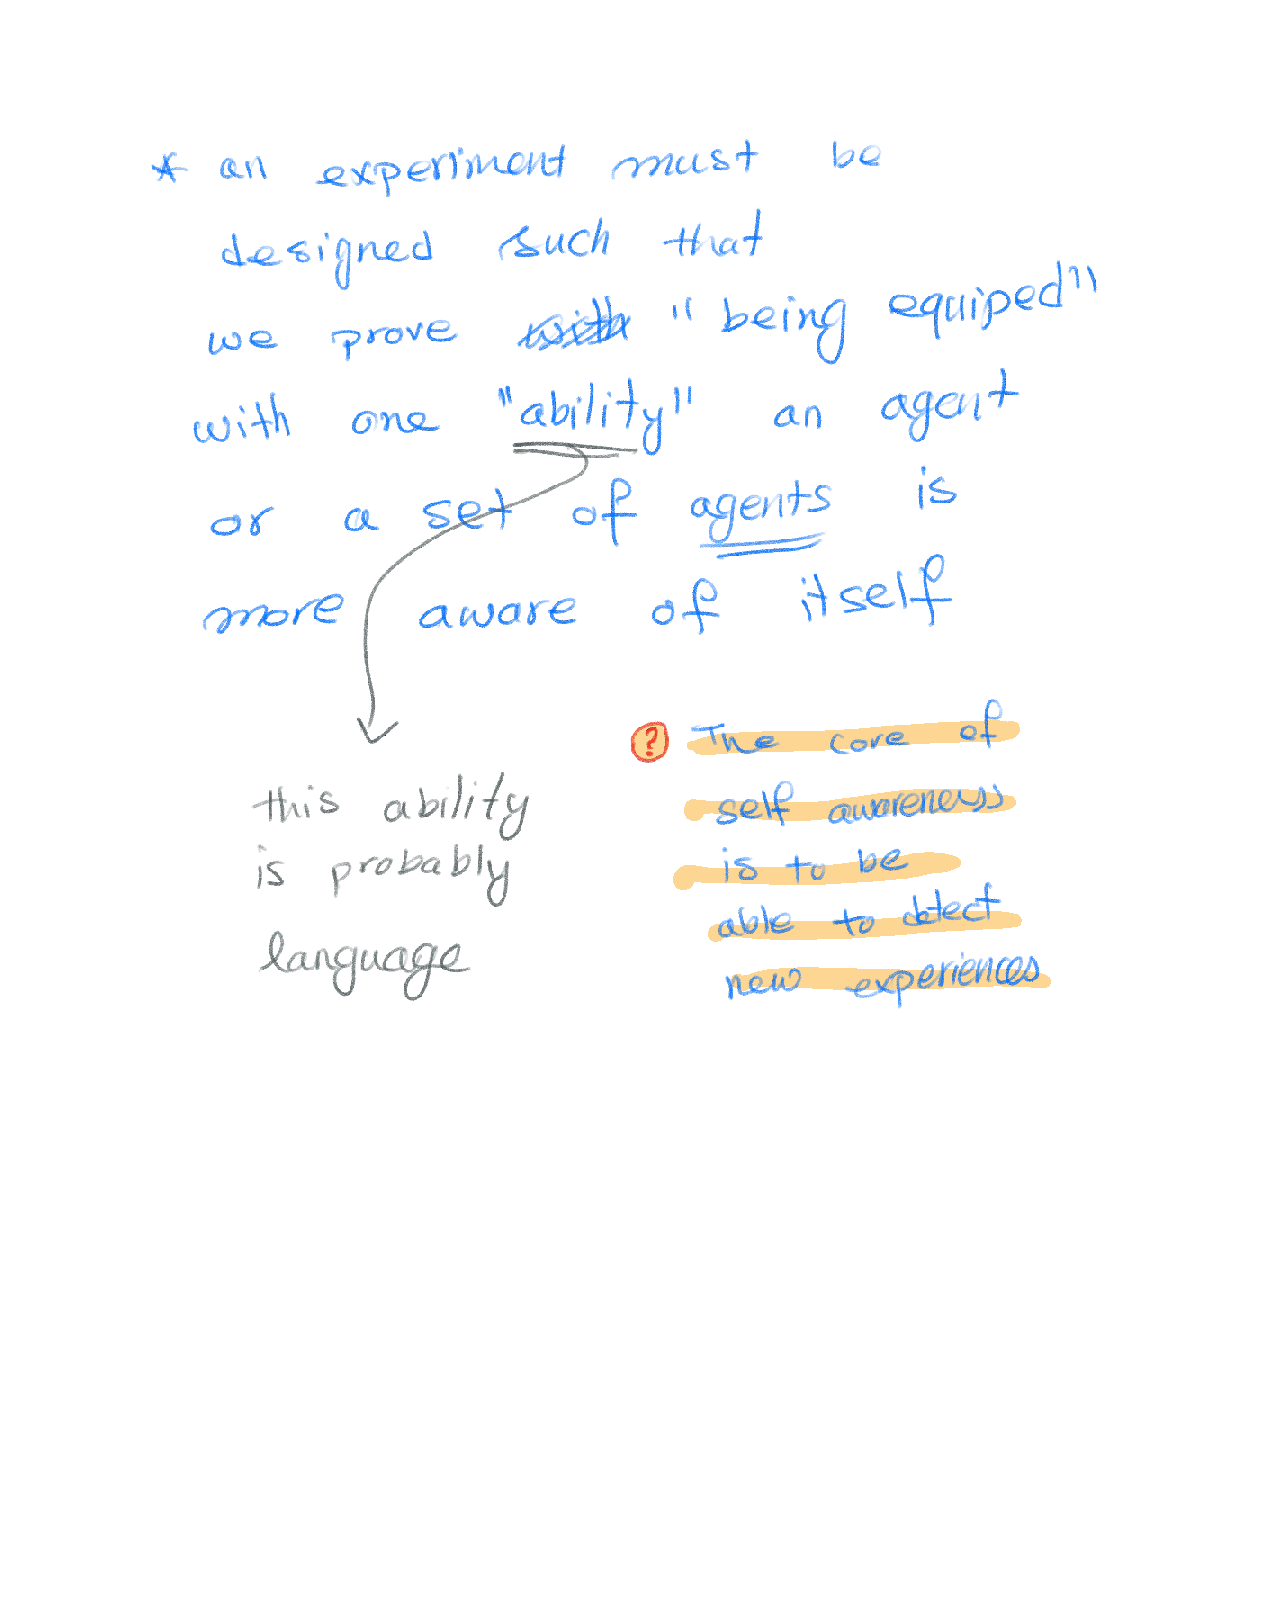
\includepdf[pages=-]{/home/donkarlo/Dropbox/repo/phd_thesis/figs/goal.pdf}


\paragraph{Main goal}
    the main goal to provide a model for language is to be able to compose different components of a language to reach newer horizens mean ing. SOme thing that human languge couldnt describe for a meaning

The goal at first stage is to propose an integrated architecture of memory
\begin{itemize}
    \item storage
    \item remember
    \item leveling (from raw )
    \item review: the process building more inner clusters (both inward and outward) and
\end{itemize}
so that it together with a time serie prediction solution it can capture the highest continous anomaly when a new experience appears in the world of the experience(s) the the robot knows.
        
        
        \begin{itemize}
            \item trying the best minimiza anomaly with language structures
        \end{itemize}